\exercise{Model Learning}
The new and improved Spinbot 2000 is a multi-purpose robot platform.
It is made of a kinematic chain consisting of a linear axis $q_{1}$, a rotational axis $q_{2}$ and another linear axis $q_{3}$, as shown in the figure below.
These three joints are actuated with forces and torques of $u_{1}$, $u_{2}$, and $u_{3}$.
Different end effectors, including a gripper or a table tennis racket, can be mounted on the end of the robot, indicated by the letter $E$.
Thanks to Spinbot's patented SuperLight technology, the robot's mass is distributed according to one point mass of $m_{1}$ at the second joint and another point mass of $m_{2}$ at the end of the robot $E$.

%\includegraphics[width=0.5\textwidth]{fig/spinbot.eps}
\colorbox{yellow}{Your graphic could be here. It just wasn't included.}

The inverse dynamics model of the Spinbot is given as
\begin{align*}
u_{1} &= (m_{1}+m_{2})(\ddot{q}_{1}+g),\\
u_{2} &= m_{2}(2\dot{q}_{3}\dot{q}_{2}q_{3}+q_{3}^{2}\ddot{q}_{2}),\\
u_{3} &= m_{2}(\ddot{q}_{3}-q_{3}\dot{q}_{2}^{2}).
\end{align*}
We now collected 100 samples from the robot while using a PD controller with gravity compensation at a rate of 500Hz.
The collected data (see \texttt{spinbotdata.txt}) is organized as follows\\
\begin{tabular}{| l || c | c | c | l  }
  \hline
   & $t_1$ & $t_2$ & $t_3$ & \ldots\\
  \hline
  \hline
  $q_{1}[m]$ &  &  &  & \\
  \hline
  $q_{2}[rad]$ &  &  &  & \\
  \hline
  $q_{3}[m]$ &  &  &  & \\
  \hline
  \ldots &  &  &  &  \\
  \hline
  $\ddot{q}_{3}[m/s^{2}]$ &  &  &  & \\
  \hline
  $u_{1}[N]$ &  &  &  & \\
  \hline
  $u_{2}[Nm]$ &  &  &  & \\
  \hline
  $u_{3}[N]$ &  &  &  & \\
  \hline
\end{tabular}

Given this data, you now want to learn the inverse dynamics of the robot in order to use a model-based controller.
The inverse dynamics of the system will be modeled as $\vec{u}=\vec{\phi}(\vec{q},\dot{\vec{q}},\ddot{\vec{q}})^{\T}\vec{\theta}$, where $\vec{\phi}(\vec{q},\dot{\vec{q}},\ddot{\vec{q}})$ are features and $\vec{\theta}$ are the parameters.

\begin{questions}

%----------------------------------------------

\begin{question}{Problem Statement}{1}
What kind of machine learning problem is learning an inverse dynamics model?

\begin{answer}
	It is a supervised learning problem. The reason being that it tries to map input to output on labelled data.
\end{answer}

\end{question}

%----------------------------------------------


\begin{question}{Assumptions}{5}
Which standard assumption has been violated by taking the data from trajectories?

\begin{answer}
	%TODO Wirkt zu einfach. Nachprüfen.
	We are not learning a function with this. This is a problem as there can be many solutions to one problem resulting in difficulties when learning (using the mean is not useful as the mean of two solutions is itself far off).
\end{answer}

\end{question}

%----------------------------------------------


\begin{question}{Features and Parameters}{4}
Assuming that the gravity $g$ is unknown, what are the feature matrix $\vec{\phi}$ and the corresponding parameter vector $\vec{\theta}$ for $\vec{u}=[u_{1},u_{2},u_{3}]^{\T}$?
(Hint: you do not need to use the data at this point)

\begin{answer}
$$\vec{\phi}=
\begin{bmatrix}
\ddot{q}_1 & 0 & 0  \\
\ddot{q}_1 & 2\dot{q}_3\dot{q}_2q_3+q_3^2\ddot{q}_2 & \ddot{q}_3-q_3\dot{q}_2^2  \\
1 & 0 & 0 
\end{bmatrix}$$
$$
\vec{\theta}= 
\begin{bmatrix} 
	m_{1} & m_{2} & g \cdot (m_{1}+m_{2})\\
\end{bmatrix}$$
\end{answer}
\end{question}


%----------------------------------------------


\begin{question}{Learning the Parameters}{2}
You want to compute the parameters $\vec{\theta}$ minimizing the squared error between the estimated forces/torques and the actual forces/torques.
Write down the matrix equation that you would use to compute the parameters. For each matrix in the equation, write down its size.\\
Then, compute the least-squares estimate of the parameters $\vec{\theta}$ from the data and report the learned values.

\begin{answer}

$\theta = (\phi\phi^{T})^{-1}\phi Y$ \\
$\theta \in \mathbb{R}^{3\times1},$\\
$\phi \in \mathbb{R}^{3\times300},$\\
$\phi^T \in \mathbb{R}^{300\times3},$\\
$Y \in \mathbb{R}^{300\times1}$\\
$\vec{\theta}= 
\begin{bmatrix} 
	-0.07297389 \\
	1.6496578 \\
	15.09510
\end{bmatrix}$
\end{answer}

\end{question}

%----------------------------------------------


\begin{question}{Recovering Model Information}{4}
	Can you recover the mass properties $m_{1}$ and $m_{2}$ from your learned parameters? Has the robot learned a plausible inverse dynamics model? Explain your answers.
	
\begin{answer}
Unfortunately, we cannot recover the mass properties from our learned parameter, since our first parameter, which denoted $m_1$, is negative. From this we deduct, that our learned parameters are not the ones we considered them to be. So the model didn't learn a plausible inverse dynamics model, but some values for the parameters so that the joints were approximated.
\end{answer}
\end{question}

%----------------------------------------------


\begin{question}{Model Evaluation}{7}
Plot the forces and torques predicted by your model over time, as well as those recorded in the data and comment the results. Is the model accuracy acceptable? If not, how would improve your model? Use one figure per joint.

\begin{answer}
	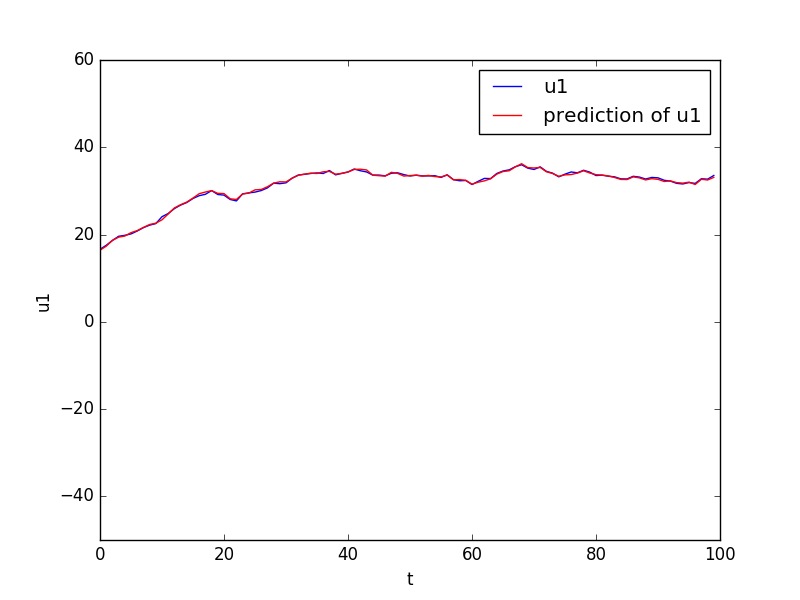
\includegraphics[width=87mm]{ML/first_joint.png}
	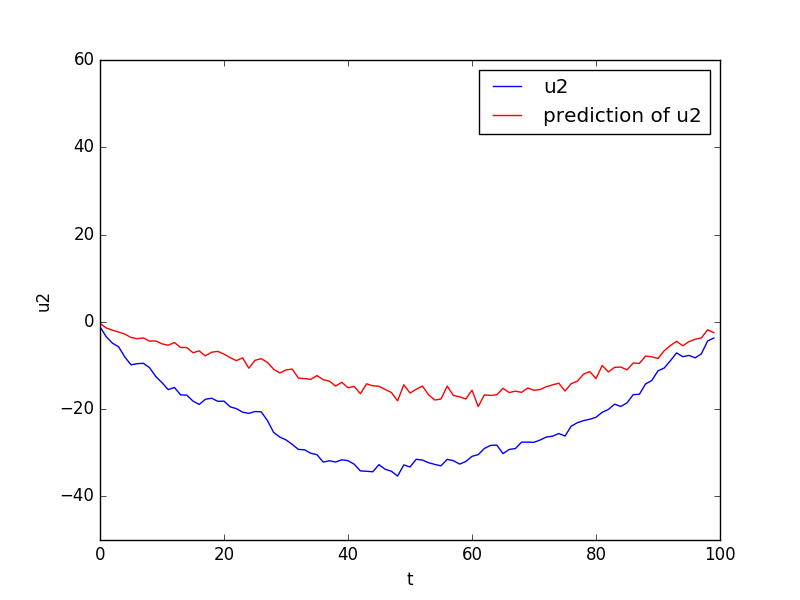
\includegraphics[width=87mm]{ML/second_joint.png}
	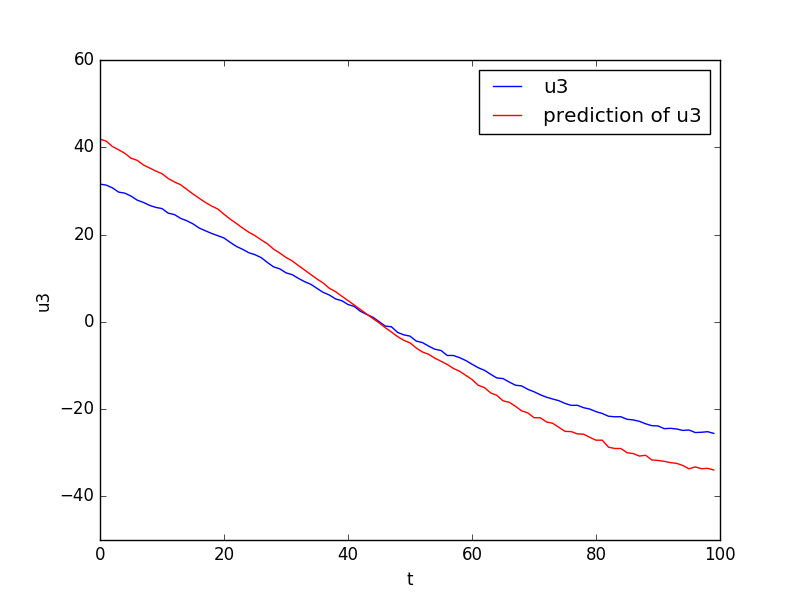
\includegraphics[width=87mm]{ML/third_joint.png}\\
	
	The prediction for the first joint is very precise.\\
	The second plot shows that the prediction for the second joint at least has the same trend as the real values, but differ especially at around half of the time.\\
	The predictions of the third joint differ at the beginning and the end the most, and are better at around half of the time. 
	All in all the models accuracy is not acceptable, since the calculated values for the second and third joints differ to much at some points.\\
	
	To improve the model, it would be better if we could integrate the gravity constant directly into the feature matrix, instead of learning it as a parameter, since it is a well known constant. Moreover, a larger dataset could be an advantage.

\end{answer}

\end{question}

%----------------------------------------------


\begin{question}[bonus]{Models for Control}{4}
Name and describe three different ways to use learned models in control laws or for generating control laws.

\begin{answer}
We can use \textbf{Controller Falsification} which uses our model to test random Control Laws and outputs the first one that does not fail.\\
We can also use it to \textbf{optimize our control law} by generating control laws and comparing them to our current best control law. \\
We can also use our learned model to \textbf{generate a policy} that simplifies our control.
\end{answer}

\end{question}

%----------------------------------------------

\end{questions}
